\documentclass[12pt]{article}
\usepackage{amsmath}
\usepackage{amssymb}
\usepackage[letterpaper,top=0.75in,bottom=1in,left=0.75in,right=0.75in,centering]{geometry}
%\usepackage{fancyhdr}
\usepackage{enumerate}
%\usepackage{lastpage}
\usepackage{multicol}
\usepackage{graphicx}

\reversemarginpar

%\pagestyle{fancy}
%\cfoot{}
%\lhead{Math 1560}\chead{Test \# 1}\rhead{May 18th, 2017}
%\rfoot{Total: 10 points}
%\chead{{\bf Name:}}
\newcommand{\points}[1]{\marginpar{\hspace{24pt}[#1]}}
\newcommand{\skipline}{\vspace{12pt}}
%\renewcommand{\headrulewidth}{0in}
\headheight 30pt

\newcommand{\di}{\displaystyle}
\newcommand{\abs}[1]{\lvert #1\rvert}
\newcommand{\len}[1]{\lVert #1\rVert}
\renewcommand{\i}{\mathbf{i}}
\renewcommand{\j}{\mathbf{j}}
\renewcommand{\k}{\mathbf{k}}
\newcommand{\R}{\mathbb{R}}
\newcommand{\aaa}{\mathbf{a}}
\newcommand{\bbb}{\mathbf{b}}
\newcommand{\ccc}{\mathbf{c}}
\newcommand{\dotp}{\boldsymbol{\cdot}}
\newcommand{\bbm}{\begin{bmatrix}}
\newcommand{\ebm}{\end{bmatrix}}                   
                  
\begin{document}


\author{Instructor: Sean Fitzpatrick}
\thispagestyle{empty}
\vglue1cm
\begin{center}
{\bf MATH 1560 - Tutorial \#7 Solutions}
\end{center}

\textbf{Additional practice:}
\begin{enumerate}
\item A person standing on a ledge $75$ m above the ground throws a ball upward at $20$ m/s. Assume that acceleration due to gravity is $-10\text{ m/s}^2$.
\begin{enumerate}
\item How high (from the ground) does the ball get?

\medskip

Let $v(t)$ denote the velocity as a function of time. The maximum height will be reached when $v(t)=0$. Since $v(0)=20$, we have $v(t) = 20-10t$, so $v(2)=0$. The ball therefore reaches its maximum height after 2 seconds.

We now need $y(t)$, the height as a function of $t$. Since $v(t)=y'(t)$ and $y(0)=75$, we get $y(t)=75+20t-5t^2$, so $y(2)=75+40-20=95$ m above the ground (20 m above the ledge).

\item How many seconds does it take before the ball hits the ground?

The ball hits the ground when
\[
x(t) = 0 = 75+20t-5t^2.
\]
The quadratic formula gives
\[
t = \frac{-20\pm \sqrt{20^2-4(-5)(75)}}{2(-5)} = 2\pm\sqrt{19}.
\]
Since $2-\sqrt{19}<0$, we must take the positive square root, giving us $t=2+\sqrt{19}\approx 6.36$ seconds. 
\end{enumerate}
\item A baseball diamond is a square with sides of length 90 feet. A baseball player hits the ball, and runs toward first base at a speed of 24 ft/s. 
\begin{enumerate}
\item At what rate is his distance from second base decreasing when he is halfway to first base?

\begin{multicols}{2}
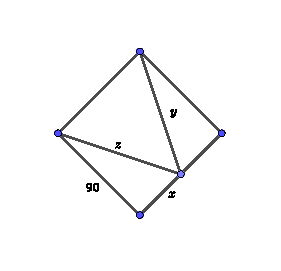
\includegraphics[width=0.9\columnwidth]{Tut7-1sol}

\columnbreak

A diagram of the situation is shown on the left. If we let $x$ denote the distance from home plate to the player, then $\dfrac{dx}{dt}=24$, and the distance from the player to first base is $90-x$.
\end{multicols}

Using the Pythagorean theorem, the distance $y$ from the player to second base satisfies
\[
y(t)^2=(90-x(t))^2+90^2,
\]
so $2y\cdot y'(t)=-2(90-x)x'(t)$. When the player is half way to first base, we have $x=45$, so $90-x=45$, and
\[
y^2=90^2+45^2=(2\cdot 45)^2+45^2=4(45^2)+45^2=5(45^2),
\]
so $y=45\sqrt{5}$, and 
\[
y'(t) = -\frac{45}{45\sqrt{5}}(24) = -\frac{24}{\sqrt{5}}.
\]
Thus, his distance from second is decreasing at a rate of $24/\sqrt{5}$ feet per second.

\item At what rate is his distance from third base increasing at the same moment?

Referring to the diagram above, we see that $z^2=x^2+90^2$, so $2z\dfrac{dz}{dt}=2x\dfrac{dx}{dt}$. When $x=45$ we get $z=45\sqrt{5}$, as above, and $\frac{dz}{dt} = \frac{24}{\sqrt{5}}$, so the distance from the player to third base is increasing at a rate of $24/\sqrt{5}$ feet per second.
\end{enumerate}
\end{enumerate}




\newpage
%\thispagestyle{empty}


\begin{enumerate}
\item An aircraft is flying away from a viewer on the ground at a speed of $210 \text{ m/s}$ at an elevation of $130 \text{ m}$. The person on the ground is watching the plane through a set of binoculars. Let $\theta$ denote the viewing angle, measured from the ground, in radians. At what rate is $\theta$ changing when the plane is $500 \text{ m}$ away (as measured along the ground)?

\begin{center}
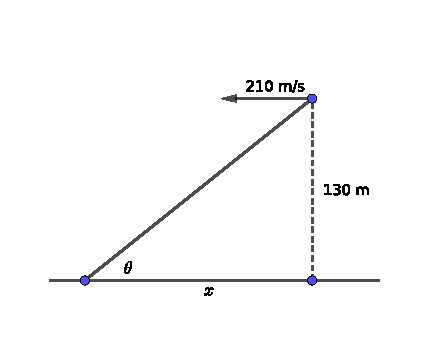
\includegraphics[width=0.5\textwidth]{Tut7-2sol}
\end{center}




A sketch of the situation is given above. From the diagram, we see that $\tan(\theta(t)) = \dfrac{130}{x(t)}$, or equivalently (and more conveniently, for derivatives), $\cot(\theta(t)) = \dfrac{x(t)}{130}$.

Taking derivatives of both sides with respect to $t$,
$
-\csc^2(\theta(t))\cdot \dfrac{d\theta(t)}{dt} = \dfrac{1}{130}\dfrac{dx(t)}{dt},
$
so \\$\dfrac{d\theta(t)}{dt} = -\dfrac{\sin^2\theta}{130}\dfrac{dx(t)}{dt}$.

Now, when $x=500$, the straight-line distance from the viewer to the plane is $\sqrt{130^2+500^2}$, and $\sin\theta = \dfrac{130}{\sqrt{130^2+500^2}}$.
Since the plane is moving away from the viewer, $x$ is increasing, so $\dfrac{dx(t)}{dt} = +210$, and we get
\[
\frac{d\theta(t)}{dt} = -\frac{1}{130}\left(\frac{130}{\sqrt{130^2+500^2}}\right)^2(210) = -\frac{130(210)}{130^2+500^2} \text{ radians per second}.
\]

\newpage

\item Suppose a police officer is 300 metres south of an intersection, and travelling north at 80 km/h. At the same time, a vehicle is 400 metres east of the same intersection, travelling east (away from the intersection). 

If the officer's radar gun registers a speed of 32 km/h, how fast is the car travelling?

\begin{center}
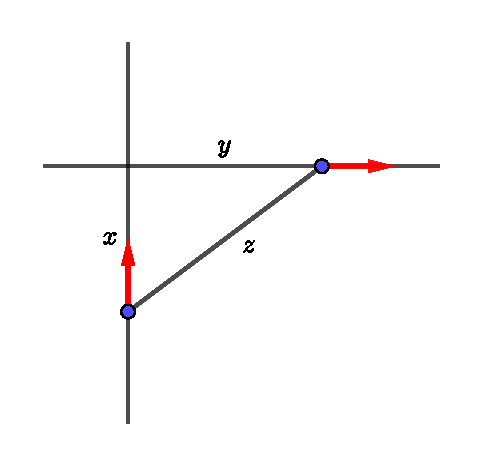
\includegraphics[width=0.5\textwidth]{Tut7-3sol}
\end{center}




A diagram of the situation is given above. The Pythagorean theorem gives us $z(t)^2=x(t)^2+y(t)^2$, so 
\[
2z(t)\cdot z'(t) = 2x(t)\cdot x'(t)+2y(t)\cdot y'(t).
\]

Since the police car is moving \textit{toward} the intersection $x$ is decreasing, so $\dfrac{dx}{dt} = -80$. 

At the time that the speed is recorded on radar, $x=300 \text{ m} = 0.3 \text{ km}$, and $y=400 \text{ m} = 0.4\text{ km}$. 

This gives us $z=0.5$ km  when the speed is registered, and the radar gun gives $\dfrac{dz}{dt} = 32$. 

Thus, we have
\[
0.4\frac{dy}{dt} = 0.5\frac{dz}{dt}-0.3\frac{dx}{dt} = 0.5(32)-0.3(-80) = 16+24=40,
\]
so $\dfrac{dy}{dt} = \dfrac{40}{0.4} = 100$ km/h.
\end{enumerate}
\end{document}